% Capítulo 3. Descripción y análisis de los datos (rúbrica: análisis de datos, 5 pts).

\section{Fuentes y filtros}
\label{sec:fuentes}

Los datos vienen de dos fuentes, ambas entregadas para el proyecto. La primera es el GTFS (\emph{General Transit Feed Specification}) de la red, que es el formato estándar para publicar horarios de transporte público y contiene las rutas, los patrones de recorrido (\texttt{trips.txt}), las frecuencias, las paradas y las geometrías con su distancia. La segunda son los archivos del enunciado, con el bus tipo y los parámetros económicos (\texttt{parameters.csv}), los electroterminales y sus plazas (\texttt{depots.csv}), los cargadores y la tarifa eléctrica por tramo horario. Se filtraron los buses de RED (\texttt{agency\_id = RM} y \texttt{route\_type = 3}), lo que deja \RutasLaboral{} de las 427 rutas; de los 26.137 registros de \texttt{trips.txt}, 14.464 son buses RED, con 839 geometrías, todas con distancia. %literal

\section{Reconstrucción de las corridas}
\label{sec:reconstruccion}

Todas las filas RED de \texttt{frequencies.txt} tienen \texttt{exact\_times = 0}, lo que significa que el archivo trae reglas de frecuencia (una salida cada cierto intervalo dentro de una ventana) y no horarios individuales. Las salidas de cada ventana se generaron como
\begin{equation}
t_n = \text{inicio} + n\cdot\text{intervalo},\qquad t_n < \text{fin},\qquad n = 0,1,2,\dots %literal
\label{eq:salidas}
\end{equation}
y cada salida hereda la duración nominal de su patrón (de la primera a la última parada) y su distancia. Cada patrón se multiplica así por las salidas de sus ventanas, y los \PatronesLaboral{} patrones laborales generan \CorridasLaboral{} corridas. La Tabla~\ref{tab:escala} resume la escala de los tres tipos de día.

\begin{table}[htbp]
\centering
\caption{Escala de la red reconstruida por tipo de día.}
\label{tab:escala}
\footnotesize
\begin{tabular}{@{}lrrrrrrr@{}}
\toprule
 & & & & Km de & & & Máximo a la vez \\
Día & Rutas & Patrones & Corridas & servicio & km/corrida & min/corrida & (hora) \\
\midrule
Laboral & \RutasLaboral & \PatronesLaboral & \CorridasLaboral & \KmServicioLaboral & \KmMedioLaboral & \DuracionMediaLaboral & \SimultaneidadLaboral{} (\HoraSimultaneidadLaboral) \\
Sábado & \RutasSabado & \PatronesSabado & \CorridasSabado & \KmServicioSabado & \KmMedioSabado & \DuracionMediaSabado & \SimultaneidadSabado{} (\HoraSimultaneidadSabado) \\
Domingo & \RutasDomingo & \PatronesDomingo & \CorridasDomingo & \KmServicioDomingo & \KmMedioDomingo & \DuracionMediaDomingo & \SimultaneidadDomingo{} (\HoraSimultaneidadDomingo) \\
\bottomrule
\end{tabular}
\fuente{Elaborada con las corridas reconstruidas (\texttt{metodo\_hibrido/instancia\_417*/corridas.csv}).}
\end{table}

\section{Cómo se mueve la red en el día}
\label{sec:curva}

La Figura~\ref{fig:corridas-dia} cuenta, cada cinco minutos, cuántas corridas están en curso. El día laboral tiene dos puntas, a las \HoraSimultaneidadLaboral{} y al atardecer, y en la de la mañana hay \SimultaneidadLaboral{} corridas a la vez. Como cada una necesita un bus distinto, ese número es una cota inferior de la flota laboral, y ningún plan puede usar menos buses. El sábado y el domingo la curva es más baja y más plana, lo que deja más tiempo libre para cargar.

\begin{figure}[htbp]
\centering
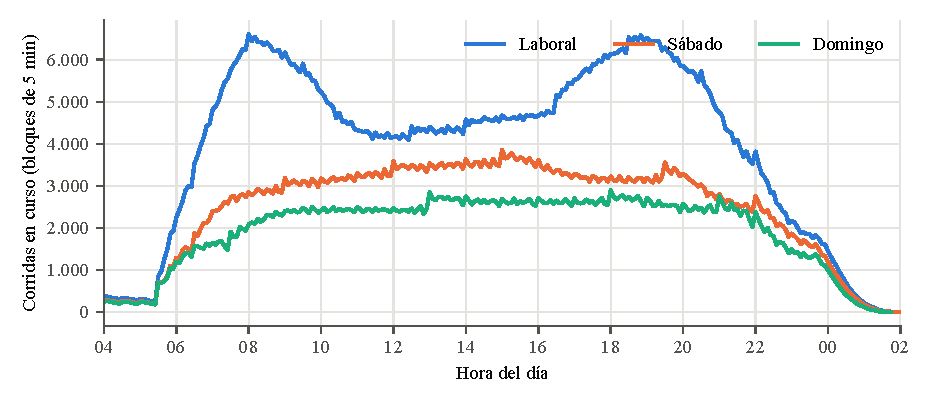
\includegraphics[width=\textwidth]{figures/corridas_dia.pdf}
\caption{Corridas en curso a lo largo del día, por tipo de día (bloques de 5 minutos).}
\label{fig:corridas-dia}
\end{figure}

Esta curva también sirvió para contrastar dos números del enunciado. La flota declarada de \FlotaDeclarada{} buses cubre apenas el \PctFlotaDeclarada\,\% de la punta laboral, de modo que no puede tomarse como límite, y el tamaño de la flota queda como decisión del modelo, tal como aclaró el equipo docente. Las \PlazasTotales{} plazas de los electroterminales también quedan muy por debajo de la flota necesaria.

\section{Energía, distancias e infraestructura}
\label{sec:energia-datos}

El consumo no viene en los datos. Se derivó de la batería y la autonomía nominal del bus, \Bateria~kWh entre \AutonomiaNominal~km, es decir \Consumo~kWh/km, igual con y sin pasajeros. Con la reserva de \PctReserva\,\%, la autonomía útil es de \Autonomia~km. A ese consumo, las corridas de un día laboral gastan \EnergiaServicioMwhLaboral~MWh.

Tampoco vienen los traslados en vacío. Se calcularon distancias viales dirigidas (sin suponer simetría ni línea recta) entre el final de cada corrida y el inicio de las demás, y entre esos puntos y los terminales y electroterminales. El tiempo de un traslado es su distancia a \VelocidadVacio~km/h, porque el enunciado no trae velocidades; las corridas mantienen su duración nominal.

Los cinco electroterminales son E1 Vespucio Norte (\PlazasUno{} plazas), E2 El Conquistador (\PlazasDos), E3 Los Espinos (\PlazasTres), E4 La Reina (\PlazasCuatro) y E5 Santa Rosa (\PlazasCinco), cada plaza con su conexión de \Potencia~kW. Para esperar y estacionar se usan cuatro terminales comunes existentes (T01 a T04), sin cargadores. La tarifa eléctrica es de USD~\TarifaMin{} por kWh de noche y sube hasta USD~\TarifaMax{} en los tramos de 14 a 17 y de 19 a 22~h.

Cada ruta se asigna al electroterminal con la menor suma de distancias por calle entre él y las cabeceras de la ruta (la salida hacia el inicio y la vuelta desde el final). Así quedan cinco sectores de \RutasSectorUno, \RutasSectorDos, \RutasSectorTres, \RutasSectorCuatro{} y \RutasSectorCinco{} rutas (Figura~\ref{fig:sectores}). El sector ordena el problema, pero los electroterminales siguen siendo compartidos por todos los buses.

\begin{figure}[htbp]
\centering
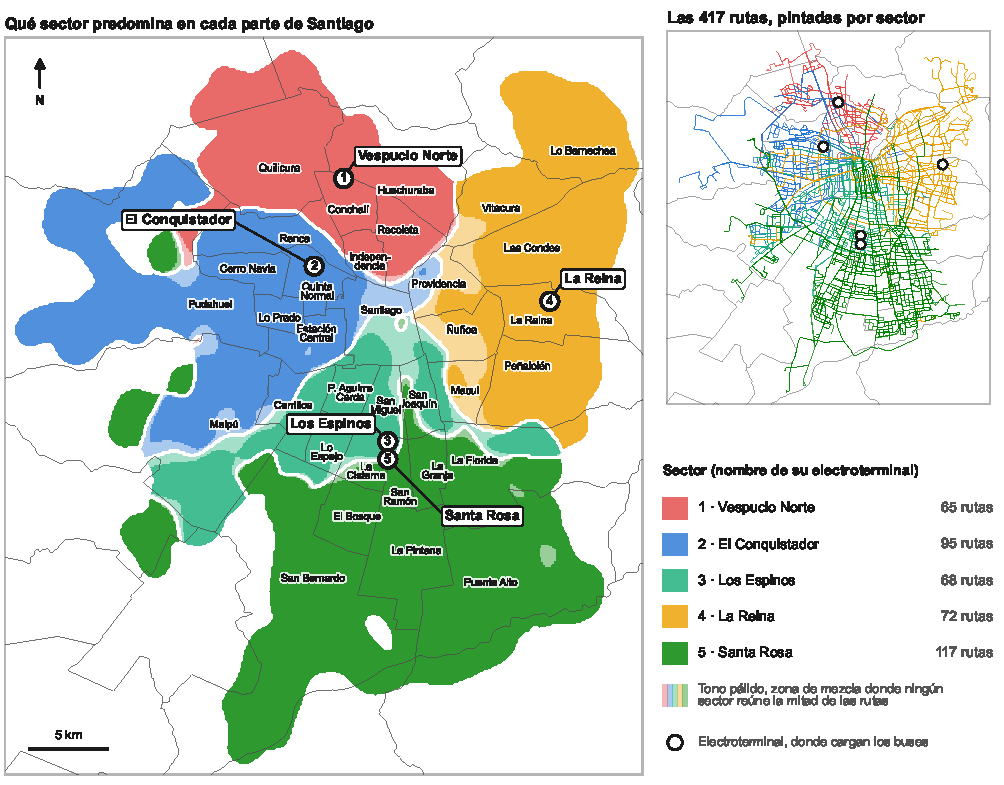
\includegraphics[width=.82\textwidth]{figures/mapa_sectores.pdf}
\caption{Sectores. Cada ruta queda asociada al electroterminal más cercano a sus cabeceras, medido por calle.}
\label{fig:sectores}
\end{figure}

\section{Datos que faltan, sesgos y cómo condicionan el modelo}
\label{sec:sesgos}

El diccionario de datos documenta \CamposDocumentados{} campos, pero \CamposAusentes{} de ellos no aparecen en ningún archivo, entre otros la potencia de los transformadores (\texttt{transformer\_mw}), los tiempos y distancias de traslado y el número de cargadores. La Tabla~\ref{tab:preparacion} resume las decisiones de preparación y cómo condicionan el modelo y los resultados.

\begin{table}[htbp]
\centering
\caption{Decisiones de preparación de los datos, riesgo de sesgo y efecto en el modelo.}
\label{tab:preparacion}
\small
\begin{tabularx}{\textwidth}{@{}p{3.6cm} X@{}}
\toprule
Decisión & Riesgo y efecto en el modelo \\
\midrule
Expandir las frecuencias (ec.~\ref{eq:salidas}) & Las salidas son representativas y no horarios observados. Fijan los huecos donde un bus puede encadenar o cargar. \\
Duraciones nominales, sin tráfico & Una conexión es factible o no, sin holgura. Con congestión, conexiones justas dejarían de serlo. Se evalúa con simulación (sección~\ref{sec:incertidumbre}). \\
Consumo lineal de \Consumo~kWh/km & Ignora pendiente, clima, pasajeros y degradación, y un error cambia directamente la flota. Se sensibiliza (sección~\ref{sec:sens-bus}). \\
Traslados a \VelocidadVacio~km/h & Define qué conexiones llegan a tiempo y cuánto cuesta reposicionar. Igual para el caso base y el método. \\
Límite eléctrico = conexiones $\times$ \Potencia~kW & El transformador no viene en los datos. Durante el día casi no se carga, así que afecta sobre todo la noche (sección~\ref{sec:repetibilidad}). \\
Terminales comunes sin límite de plazas & El enunciado no da su capacidad, y con un límite algunos buses terminarían más lejos (sección~\ref{sec:supuestos}). \\
Día aislado con batería llena & Lo fija el enunciado para ambos planes y favorece planes que terminan con poca energía (sección~\ref{sec:repetibilidad}). \\
Sectores fijos & Reduce el tamaño de cada búsqueda y evita cruzar la ciudad, pero impide combinar corridas de sectores vecinos. \\
\bottomrule
\end{tabularx}
\end{table}

Ninguna de estas decisiones favorece al método frente al caso base, porque ambos usan las mismas corridas, distancias, velocidad, terminales y batería inicial. Sí condicionan la lectura de los resultados, porque los planes son factibles dentro del modelo y no necesariamente en la operación real (capítulos~\ref{ch:sensibilidad} y~\ref{ch:piloto}).
